\documentclass[12pt]{amsart}

\usepackage{amssymb}
\usepackage{tikz}
\usetikzlibrary{matrix,arrows}
\usepackage{amsrefs}

\begin{document}

Let $R$ be polynomial ring and let
\begin{center}
  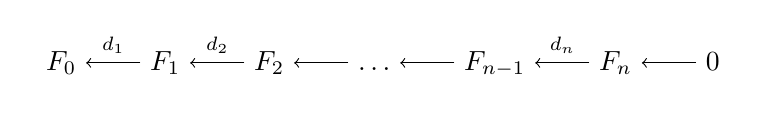
\begin{tikzpicture}[description/.style={fill=white,inner sep=2pt}]
    \matrix (m) [matrix of math nodes, row sep=5em,
    column sep=2em, text height=1.5ex, text depth=0.25ex]
    { F_0 & F_1 & F_2 & \dots & F_{n-1} & F_n & 0\\ };
    \path[->,font=\scriptsize]
    (m-1-2) edge node[above] {$d_1$} (m-1-1);
    \path[->,font=\scriptsize]
    (m-1-3) edge node[above] {$d_2$} (m-1-2);
    \path[->,font=\scriptsize]
    (m-1-4) edge node[above] {} (m-1-3);
    \path[->,font=\scriptsize]
    (m-1-5) edge node[above] {} (m-1-4);
    \path[->,font=\scriptsize]
    (m-1-6) edge node[above] {$d_n$} (m-1-5);
    \path[->,font=\scriptsize]
    (m-1-7) edge node[above] {} (m-1-6);
  \end{tikzpicture}
\end{center}
be an acyclic complex of free $R$-modules.  Let $f_k$ denote the rank
of the module $F_k$ and let $r_k$ denote the rank of $d_k$.  By the
Buchsbaum-Eisenbud exactness criterion, $r_{k+1}+r_k = f_k$. For
$1\leqslant k\leqslant n$, the $a$-multipliers are maps of graded
$R$-modules
\begin{equation*}
  a_k \colon R(-u_k) \longrightarrow \bigwedge^{r_k} F_{k-1}.
\end{equation*}
defined recursively as follows. The map $a_n$ is the exterior power
map
$\bigwedge^{r_n} d_n \colon \bigwedge^{r_n} F_n \to \bigwedge^{r_n}
F_{n-1}$, so $\bigwedge^{r_n} F_n \cong R(-u_n)$ where $u_n$ is the
sum of the degrees of the elements in a basis of $F_n$.  For $k<n$,
$a_k$ is defined to make the following diagram commutative:
\begin{center}
  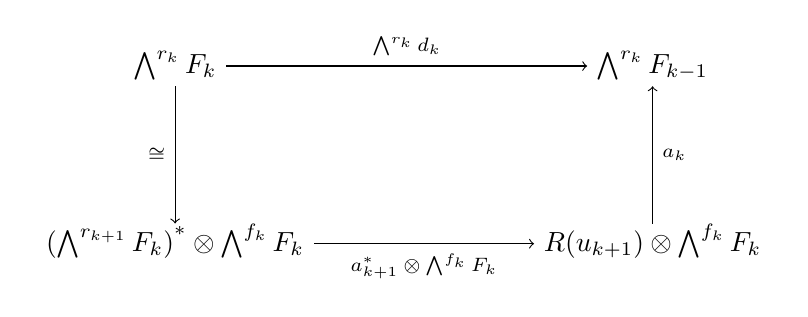
\begin{tikzpicture}[description/.style={fill=white,inner sep=2pt}]
    \matrix (m) [matrix of math nodes, row sep=5em,
    column sep=8em, text height=1.5ex, text depth=0.25ex]
    { \bigwedge^{r_k} F_k & \bigwedge^{r_k} F_{k-1} \\
      \left(\bigwedge^{r_{k+1}} F_k \right)^* \otimes \bigwedge^{f_k} F_k & R(u_{k+1}) \otimes \bigwedge^{f_k} F_k \\ };
    \path[->,font=\scriptsize]
    (m-2-2) edge node[right] {$a_k$} (m-1-2);
    \path[<-,font=\scriptsize]
    (m-1-2) edge node[above] {$\bigwedge^{r_k} d_k$} (m-1-1);
    \path[<-,font=\scriptsize]
    (m-2-1) edge node[left] {$\cong$} (m-1-1);
    \path[<-,font=\scriptsize]
    (m-2-2) edge node[below] {$a_{k+1}^* \otimes \bigwedge^{f_k} F_k$} (m-2-1);
  \end{tikzpicture}
\end{center}
where the vertical arrow at the left is the exterior duality
isomorphism induced by the perfect pairing
$\bigwedge^{r_k} F_k \otimes \bigwedge^{r_{k+1}} F_k \to
\bigwedge^{f_k} F_k$. It follows that
$R(-u_k) \cong R(u_{k+1}) \otimes \bigwedge^{f_k} F_k$. The existence
of these multipliers was proved by in \cite[Theorem 3.1]{MR340240}.

Next we define lower order multipliers, whose existence was conjecture in \cite[Conjecture 10.1]{MR340240} and proved in \cite[Theorem 2]{MR540642}. First define maps $a^j_k \colon R(-u_k) \otimes \bigwedge^j F_{k-1} \to \bigwedge^{r_k+j} F_{k-1}$ via the composition
\begin{center}
  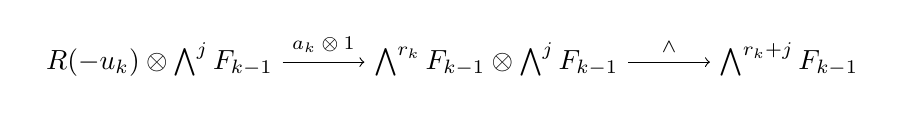
\begin{tikzpicture}[description/.style={fill=white,inner sep=2pt}]
    \matrix (m) [matrix of math nodes, row sep=5em,
    column sep=3em, text height=1.5ex, text depth=0.25ex]
    { R(-u_k) \otimes \bigwedge^j F_{k-1} & \bigwedge^{r_k} F_{k-1} \otimes \bigwedge^{j} F_{k-1} & \bigwedge^{r_k+j} F_{k-1} \\ };
    \path[->,font=\scriptsize]
    (m-1-1) edge node[above] {$a_k \otimes 1$} (m-1-2);
    \path[->,font=\scriptsize]
    (m-1-2) edge node[above] {$\wedge$} (m-1-3);
  \end{tikzpicture}
\end{center}
where the second map is exterior multiplication. For all $j$ such that $(j-1)n\leqslant j(k-1)-2$, there exists a map $c^j_k \colon R(-u_{k-1}) \otimes \bigwedge^j F_{k-1} \to \bigwedge^{r_{k-1}-j} F_{k-2}$ that makes the following diagram commutative:
\begin{center}
  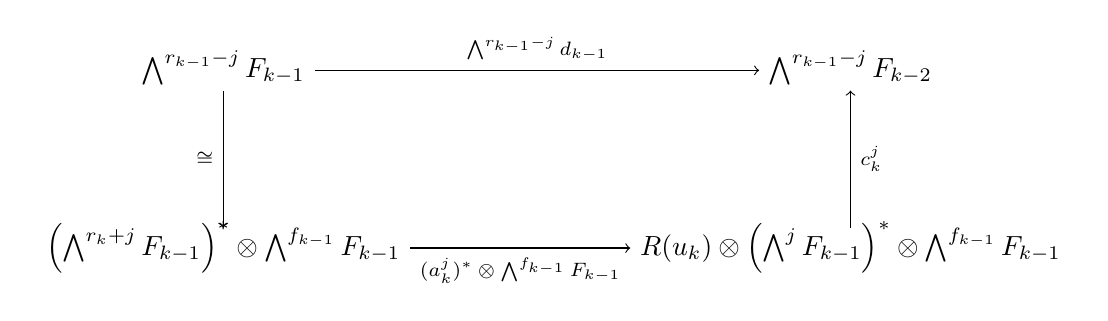
\begin{tikzpicture}[description/.style={fill=white,inner sep=2pt}]
    \matrix (m) [matrix of math nodes, row sep=5em,
    column sep=8em, text height=1.5ex, text depth=0.25ex]
    { \bigwedge^{r_{k-1}-j} F_{k-1} & \bigwedge^{r_{k-1}-j} F_{k-2} \\
      \left(\bigwedge^{r_k+j} F_{k-1} \right)^* \otimes \bigwedge^{f_{k-1}} F_{k-1} & R(u_k) \otimes \left( \bigwedge^j F_{k-1} \right)^* \otimes \bigwedge^{f_{k-1}} F_{k-1} \\ };
    \path[->,font=\scriptsize]
    (m-2-2) edge node[right] {$c^j_k$} (m-1-2);
    \path[<-,font=\scriptsize]
    (m-1-2) edge node[above] {$\bigwedge^{r_{k-1}-j} d_{k-1}$} (m-1-1);
    \path[<-,font=\scriptsize]
    (m-2-1) edge node[left] {$\cong$} (m-1-1);
    \path[<-,font=\scriptsize]
    (m-2-2) edge node[below] {$(a^j_k)^* \otimes \bigwedge^{f_{k-1}} F_{k-1}$} (m-2-1);
  \end{tikzpicture}
\end{center}
where the vertical arrow at the left is the exterior duality
isomorphism.


\begin{bibdiv}
\begin{biblist}

\bib{MR340240}{article}{
   author={Buchsbaum, David A.},
   author={Eisenbud, David},
   title={Some structure theorems for finite free resolutions},
   journal={Advances in Math.},
   volume={12},
   date={1974},
   pages={84--139},
   issn={0001-8708},
   review={\MR{340240}},
   doi={10.1016/S0001-8708(74)80019-8},
}

\bib{MR540642}{article}{
   author={Weyman, Jerzy},
   title={Resolutions of the exterior and symmetric powers of a module},
   journal={J. Algebra},
   volume={58},
   date={1979},
   number={2},
   pages={333--341},
   issn={0021-8693},
   review={\MR{540642}},
   doi={10.1016/0021-8693(79)90164-9},
 }
 
\end{biblist}
\end{bibdiv}

\end{document}

%%% Local Variables:
%%% mode: latex
%%% TeX-master: t
%%% End:
